\documentclass[a4paper,12pt,twoside,english]{article}

\usepackage{times}  
\usepackage{amsmath}
\usepackage{amssymb}
\usepackage{graphicx}
\usepackage{wrapfig}
\usepackage{theorem}
\usepackage[latin1]{inputenc}
\usepackage{latexsym}
\usepackage{url}
\usepackage[english]{babel}
\usepackage{subcaption}
\usepackage{caption}

\headsep          0.25in
\headheight       12pt
\setlength{\topmargin}{-\headsep}
\addtolength{\topmargin}{-\headheight}
%\oddsidemargin      0in
\evensidemargin 0in
\setlength{\textwidth}{\paperwidth}
\addtolength{\textwidth}{-2.0in}
\setlength{\textheight}{\paperheight}
\addtolength{\textheight}{-2.0in}
\addtolength{\textheight}{-1\topskip}
\divide\textheight  by \baselineskip
\multiply\textheight  by \baselineskip
\addtolength{\textheight}{\topskip}


\title{Angry Cuts}
%\date{2014-02-13}
\author{Anton Alb\`{e}rt Karlstr\"{o}m, Lovisa Dahl, \\Emma Edvardsson
 and Hannes Ingelhag, \\Norrk\"{o}ping}

%Gör så att alla formler blir lite större
\everymath{\displaystyle}

\begin{document}

%\pagestyle{empty}

%----------------------------- Front matter of the document

\begin{figure}
\begin{center}

\includegraphics[width=6cm]{bilder/LiTH_sigill_col.png} 
\end{center}
\end{figure}

\maketitle
\pagenumbering{gobble}

\newpage
\begin{abstract}
Write an abstract here!
\vfill
\end{abstract}

%\tableofcontents  % chapter with the table of contents
%\addtocontents{toc}{\protect\thispagestyle{empty}}
%\listoffigures    % chapter with the list of figures
%\addtocontents{lof}{\protect\thispagestyle{empty}}
%\listoftables     % chapter with the list of tables
%\addtocontents{lot}{\protect\thispagestyle{empty}}

%----------------------------- Body of the document
\newpage

\pagenumbering{arabic}
\pagestyle{plain}


\setcounter{page}{1}
\section{Introduction}
\subsection{Background}
Angry cuts is a project of modeling and simulating the scenario of a weight attached to a pendulum converting to a projectile in two dimensions. 
The final concept is a simulation of several weights, each attached to a pendulum. All the ropes are being cut at the same time which results in projectile movement for all the weights. In this state the weights are interacting with both the walls and each other.

Figure 1 shows the first idea, where a pendulum is supposed to hit a tower of wooden bars. The projectile movement is inspired by the slingshot aiming towards a given target in the game {\itshape Angry birds}. The idea of releasing a weight from a pendulum is claimed from {\itshape Cut the rope}. In order to create a scene with real physics, the collisions in the scene require careful calculation of the collisions, both with static and dynamic objects. Since objects in equilibrium are difficult to handle in simulation, the idea was modified to have the weights alone acting in a room with walls and floor, and extend with several balls instead of the wooden bars. The definitive idea is illustrated in Fig. 2, the scene consists of a pendulum in a room, which later will be released as a projectile.


\begin{figure}[h]
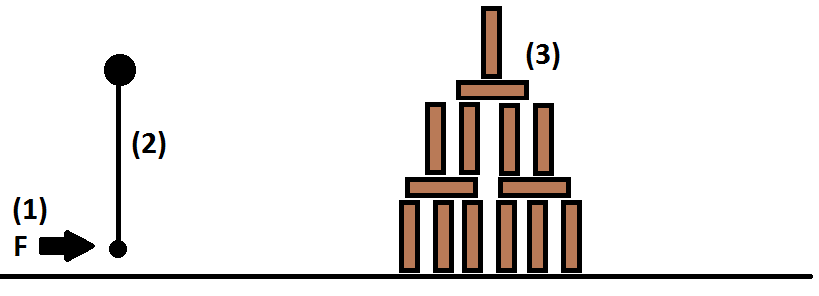
\includegraphics[height=3.5cm]{bilder/ideasketch.png}
\centering
\caption{Original idea}
\end{figure}
\begin{figure}[h]
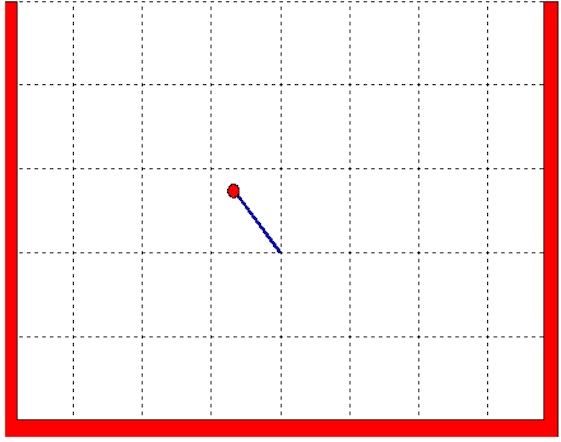
\includegraphics[height=4cm]{bilder/Matlab_Pendulum1.png}
\centering
\caption{Modified idea}
\end{figure} 



\subsection{Purpose}
The purpose of this report is to describe and follow the development of the scene with pendulums, projectiles and collisions in two dimensions. The scene uses physically correct models and formulas for collisions with static and dynamic objects. Air resistance and energy loss are taken in consideration in the pendulum, the projectile and the collision.

Another purpose with this project is to use Matlab to test and develop the model before transferring the model into C++ and OpenGL. 

\section{Physical model}
The first part of this project was to find the physical description of the first two parts of the model: the pendulum and the projectile movement. The second part was to implement collision handler and air resistance. 
\subsection{Pendulum}
A physical model of a nonlinear pendulum (1) was required since the system operates with large angles. \cite{Nor:06} \cite{Hal:10} \\ \\
$\frac{d^2\theta}{dt^2} + \frac{g}{L}*sin(\theta(t)) = 0$ \hfill (1) \\ 
Figure 3 illustrates the model of the pendulum, $g$ represents the gravity constant, $L$ the length of the rope of the pendulum and $\theta$ is the angle of the pendulum perpendicular to the gravity.  $\frac{d^2\theta}{dt^2}$, the angular acceleration, is the relationship between the position of the weight and the angle perpendicular to gravity.

 \begin{table}[h!]
  \centering
  \begin{tabular}{c  c}
        \begin{minipage}{0.5\textwidth}
      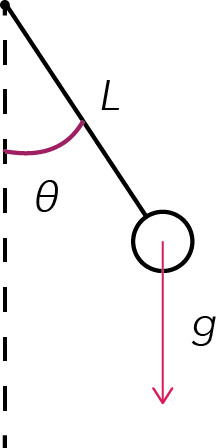
\includegraphics[height=60mm]{bilder/pendulum_2.png}
      \centering
%      \captionsetup{justification=raggedright, singlelinecheck=false}
      \captionof{figure}{Physical model of a pendulum}
    \end{minipage}
    & 
  \begin{minipage}{0.5\textwidth}
      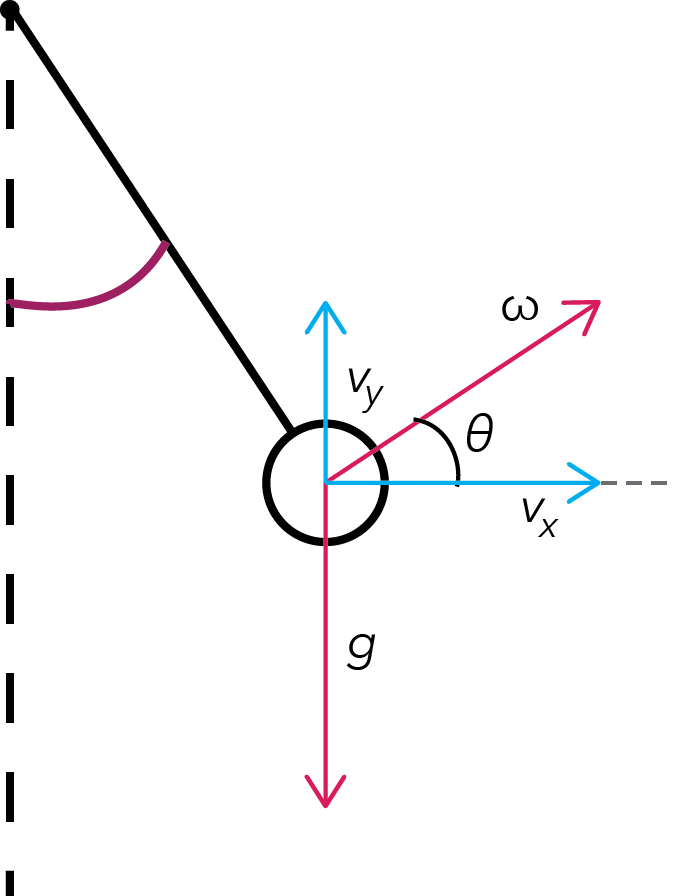
\includegraphics[height=60mm]{bilder/projectile_dynamics.png}
     \centering
      \captionsetup{justification=raggedright, singlelinecheck=false}
      \captionof{figure}{Initial dynamics of the projectile}
    \end{minipage} \\
  \end{tabular}
\end{table}

\subsection{Projectile}
When the rope was cut, the outcoming velocity from the pendulum movement was captured as the initial velocity for the projectile movement. In order to transfer the movement into projectile, illustrated in Fig. 4, the velocity was split into horizontal (2) and vertical velocity (3). The angle ${\theta_i}$ between the velocity vector and the horizon determined the magnitude of $v_x(t)$ and $v_y(t)$. The acceleration (4) was derived with the same method, although the vertical velocity, which also gravity was acting on. 
 \\ \\
$v_x(t) = v_{out}(t) * cos(\theta_i(t))$ \hfill (2) \\
$v_y(t) = v_{out}(t) * sin(\theta_i(t))$ \hfill (3) \\
$a_y(t) = a_{out}(t) * sin(\theta_i(t)) - g$ \hfill (4) \\


 
\subsection{Air resistance}
To add air resistance to the model, the velocity should be reduced according to the angle perpendicular to the gravity. The air resistance (5) was calculated using the density of air ${\rho}$, the drag coefficient of a sphere $c_d$, the cross sectional area {\itshape A}  of the object and the velocity, $v$ of the weight.
The air resistance was added to affect the velocity decreasingly which was performed by appending the $F_d$ to $v_y$ in (3).\\ \\
$F_d = \frac{1}{2}( \rho * v^2(t) * c_{d} * A)$ \hfill (5) 

\subsection{Collision detection}
\subsubsection{Collision with walls and floor}
The second part of the model was to consider the collisions with walls and floor. This was performed by changing the direction after the collision according to the normal of the surface hit by the weight. The velocity was reduced with 50\%  to simulate an energy loss from the collision.  Equation 6 and 7 simulates a collision between the west wall and our weight. In equation 7 the $x_{weight}$ is the x-position of the weight, $x_{wall}$ the x-position of the west wall and r the weights radius.  \\ \\
$v_x= -0.5*v_x$ \hfill (6) \\
$x_{weight} = x_{wall}+ r$ \hfill (7)

\subsubsection{Collision between objects}
The third physical part in the system was collision between two moving objects. In this project all collisions are considered elastic, which means that the objects cannot stick together in the collision.
A collision is detected when the distance between two weights is smaller than the sum of the radii. The distances can be calculated using Pythagorean theorem, illustrated in Fig. 5. 
Since a numerical method is used to calculate the next step of the scene, the weights might overlap, step 1 Fig. 6, and due to that get stuck to each other, an unwanted phenomena. To get a more realistic simulation of the collision, the boundaries of the weights must intersect instead of overlap. Therefore, when a collision is detected, the weights are set to their previous positions, step 2 Fig. 6, and from there smaller steps in the same direction are taken until they intersect, Fig. 6. 

\begin{table}[h!]
  \centering
  \begin{tabular}{c}
        \begin{minipage}{0.5\textwidth}
      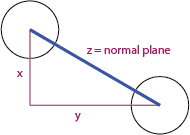
\includegraphics[height=3.1cm]{bilder/pythagora.png} 
      \centering
   \captionof{figure}{Distance between two weights\\ using the pythagorean theorem \\} 
    \end{minipage} 
 \\
  \begin{minipage}{0.5\textwidth}
      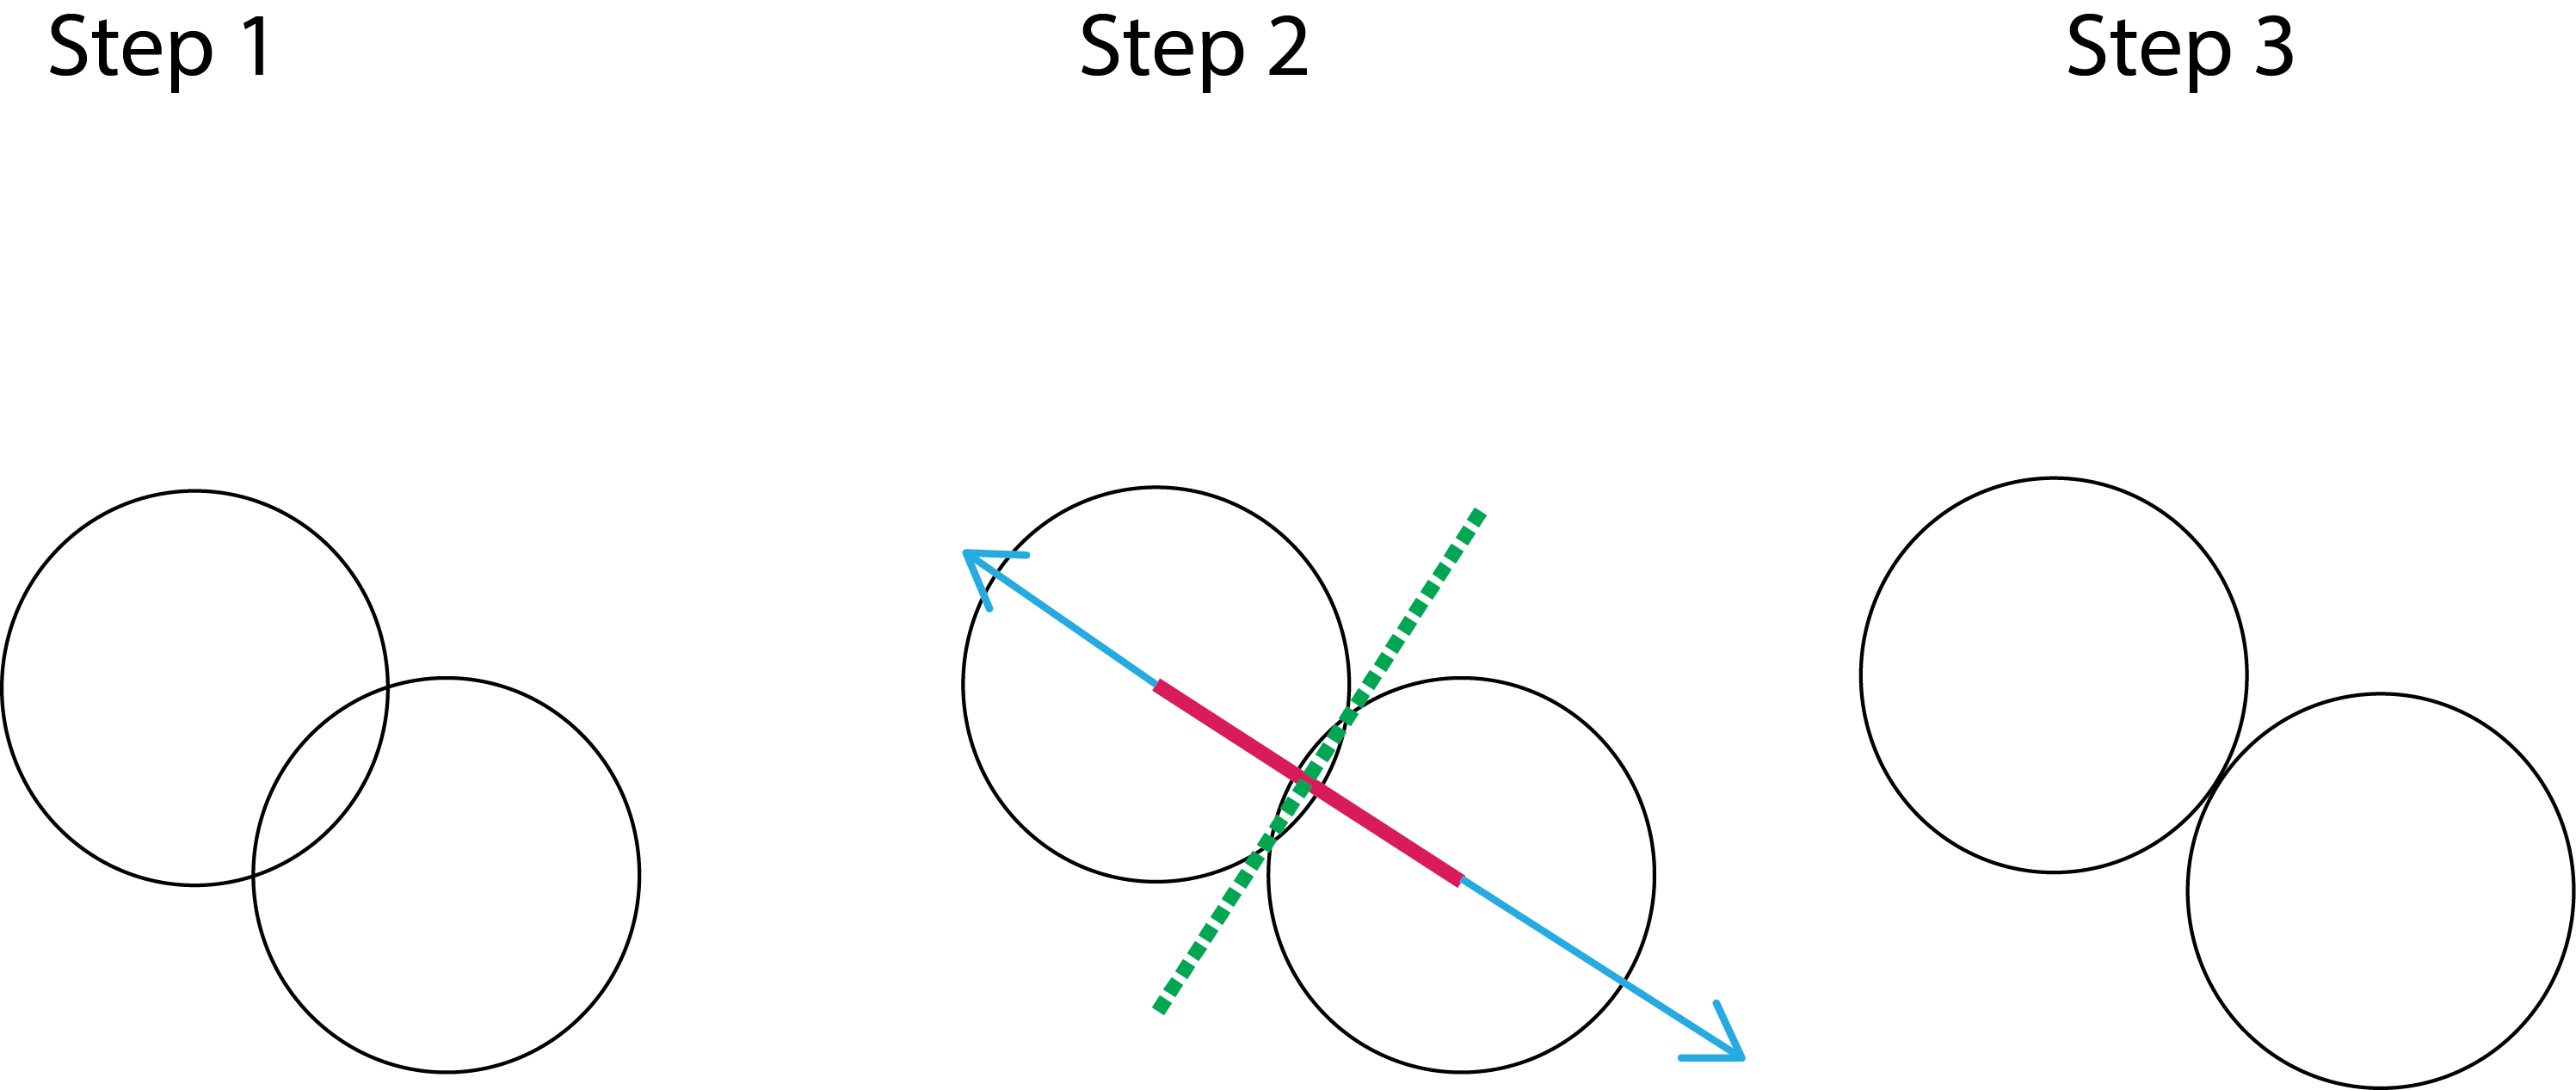
\includegraphics[height=3.2cm]{bilder/Collision_management.png}
      \centering
     \captionof{figure}{\\ \textit{Step 1:} Overlapping weights \\ \textit{Step 2}: Collision and normal planes are found \\ \textit{Step 3:} Collision can now be calculated}
    \end{minipage} 
    \end{tabular}
\end{table}

To calculate the direction of the weights after the collision, the normal plane of the weights is used. This can be determined as the distance between center points of the weights. A collision plane is calculated by the normal plane, as illustrated in Fig. 7. 

The initial velocity vectors can now be described in the normal- and the collision plane, Fig 8. These vectors can be obtained by the operation vector dot product. When these vectors are found the new velocity vector after the collision can be determined according to 6 and 7.  \\ \\
$ v_{1a}(t) = \frac{1}{m_1+m_2}*(v_1(t)(m_1-m_2) + 2m_2*v_2(t)) $ \hfill (6) \\ \\
$ v_{2a}(t) = \frac{1}{m_1+m_2}*(v_2(t)(m_2-m_1) + 2m_1*v_1(t))$ \hfill (7) \\ \\

$v_{1a}(t)$ and $v_{2a}(t)$ denotes the velocity of the weights, respectively, after the collision, $m_1$ and $m_2$ describes the masses of the colliding weights. $v_1$ and $v_2$ are the velocities of the weights before the collision. 

\begin{table}[h!]
  \begin{tabular}{c c}
    \begin{minipage}{0.5\textwidth}
      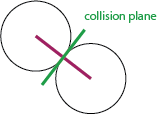
\includegraphics[height=3cm]{bilder/collisionplane.png}
      \centering
      \captionof{figure}{Collision plane}
    \end{minipage}
    &
  \begin{minipage}{0.5\textwidth}
      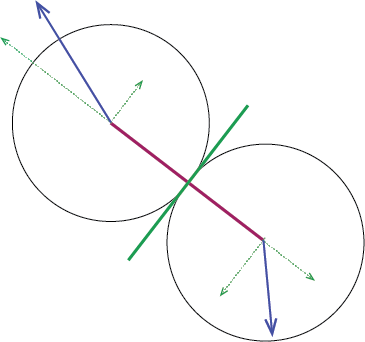
\includegraphics[height=3cm]{bilder/newvelocitiesvectors_new.png}
      \centering
      \captionof{figure}{Modified idea}
    \end{minipage} \\
  \end{tabular}
\end{table}

\subsection{Numerical implementation}
\subsubsection{Euler's explicit method}
Euler$'$s explicit method (8) is used to calculate the x and y position of the weight and the angular velocity continuously over time of the nonlinear pendulum. \\ \\
$y(t + h) = y(t) + f(t,y(t))*h$  \hfill (8) \\

In (8), $h$ denotes the step length, $y(t)$ is the function and $f$ describes the derivative of $y$.
\subsubsection{Runge-Kutta method}
Runge-Kutta is another numerical method. Compared to Euler it gives a more stable system and can be used with a larger step size. The most common form of the Runge-Kutta is RK4, a fourth order method, which is described in (9).\\ \\
$k_1 = h*f(x_i, y_i) $ \\ \
$k_2 = h*f(x_i + 0.5*h, y_i + 0.5*k_1) $ \\
$k_3 = h*f(x_i + 0.5*h, y_i + 0.5*k_2)$ \hfill (9) \\
$k_4 = h*f(x_i + h, y_i + k_3)$ \\

By using these four equations the next step can be calculated according to (10). \\ \\
$ y(i+1) = y(i) + \frac{1}{6}( k_1 + 2*k_2 + 2*k_3 + k_4) $ \hfill (10)

\subsection{Graphical implementation}
\subsubsection{MATLAB}
A physical model of one weight was defined and implemented in MATLAB for a simulation test. Constants for the calculations can be found in \textit{Appendix 1}. This was made iteratively, starting with the pendulum alone followed by adding the projectile movement and the last step with collision detection with static objects. The final simulation consisted of a weight attached to a pendulum, see Fig. 9, which was released after a given time and converted into a projectile. The weight would bounce on the walls and the ground until the added energy loss caused it to stop moving. 

The second part was to add interaction between two weights in the same room. This step required a fully working model of one weight and an additional collision management to handle collision between two dynamic objects. Fig. 10 shows two weights of different radii.

\begin{table}[h!]
  \centering
  \begin{tabular}{c  c}
        \begin{minipage}{0.5\textwidth}
      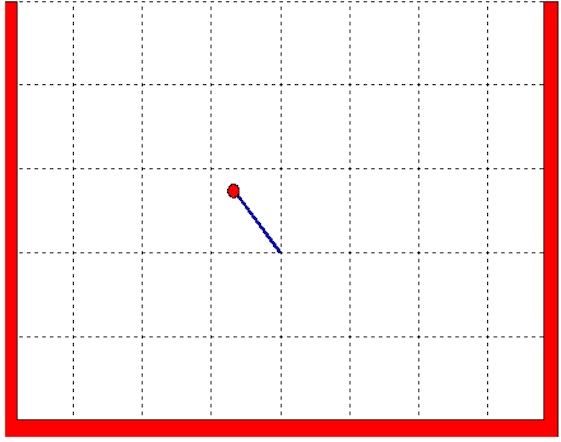
\includegraphics[width=\linewidth, width=60mm]{bilder/Matlab_Pendulum1.png}
      \centering
%      \captionsetup{justification=raggedright, singlelinecheck=false}
      \captionof{figure}{Plot of one pendulum}
    \end{minipage}
    & 
  \begin{minipage}{0.5\textwidth}
      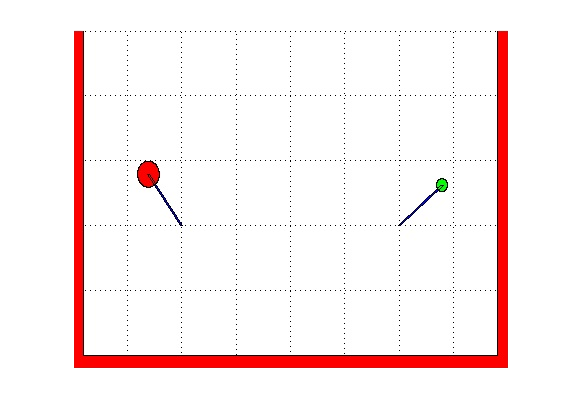
\includegraphics[width=\linewidth, width=60mm]{bilder/Matlab_Pendulum2.png}
%      \centering
      \captionsetup{justification=raggedright, singlelinecheck=false}
      \captionof{figure}{Plot of two pendulums}
    \end{minipage} \\
  \end{tabular}
\end{table}



\subsubsection{OpenGL 3.3}
To improve the graphical representation of the model the code was converted to C++ and OpenGL. The software used in the project were Sublime Text 2, Visual Studio and CMake. 

A possibility to change the number of weights in the scene was implemented, in such way that the pendulums were drawn with even intervals according to the number of weights. Fig. 11 and Fig. 12 presents the scene with three weights in OpenGL. The constants used for these figures are the same as previous.

\begin{table}[h!]
  \centering
   \begin{tabular}{c c}
      \begin{minipage}{0.5\textwidth}
      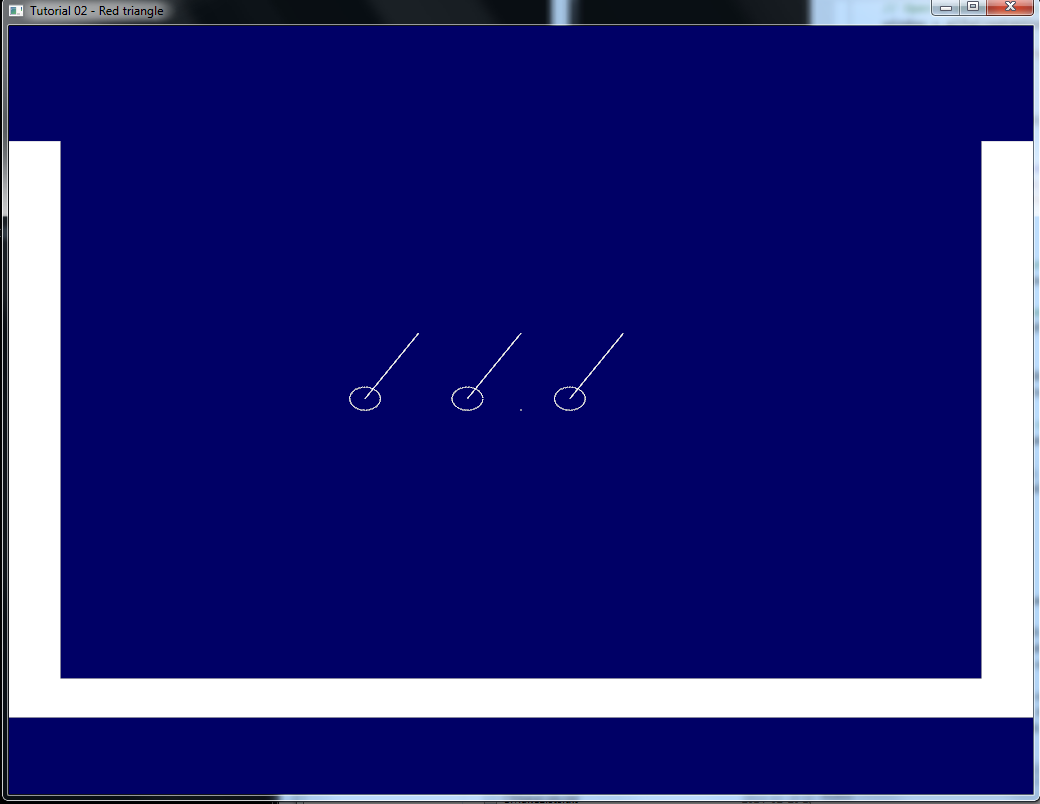
\includegraphics[width=\linewidth, width=60mm]{bilder/OpenGL_pendulum0.png}
      \centering
      \captionof{figure}{Simulation of three pendulums, first version}
   \end{minipage}
    & 
   \begin{minipage}{0.5\textwidth}
   \vspace{1.8cm}
     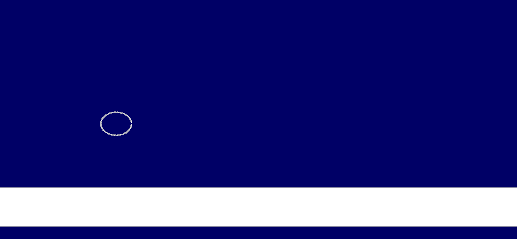
\includegraphics[width=\linewidth, width=60mm]{bilder/OpenGL_bounce0.png}
     \centering
     \captionof{figure}{One projectile, first version}
    \end{minipage} \\
  \end{tabular}
\end{table}

\section{Result}
The result retrieved from this project is a program where the user could enter the desired number of pendulums in a GUI. The trigger of movement for the pendulums are their initial angle given by the user or in program. During the execution of the program the user could follow the flow of energy in the scene. The weights are positioned depending on the given number and are set to a random color. In Fig. 13 and Fig. 14 seven weights are implemented.

\begin{table}[h!]
  \centering
   \begin{tabular}{c c}
    \begin{minipage}{0.5\textwidth}
      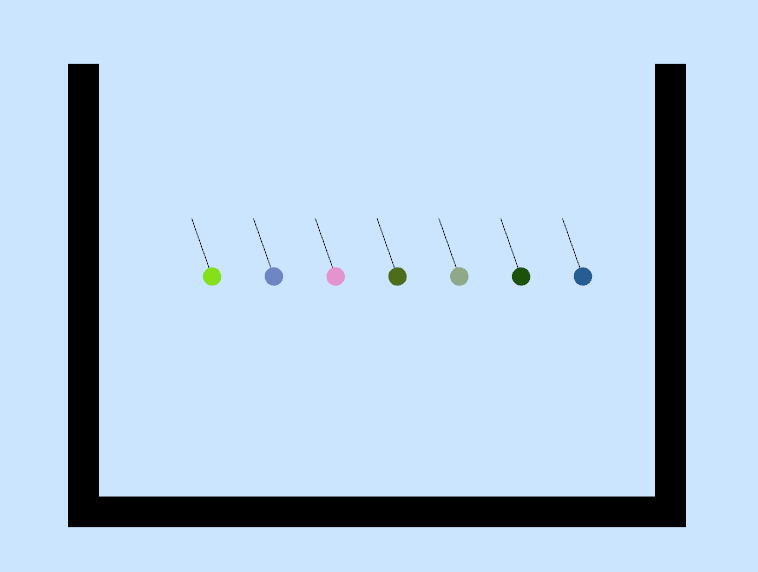
\includegraphics[width=\linewidth, width=60mm]{bilder/OpenGL_pendulum1.png}
      \centering
      \captionof{figure}{Seven weights simulated in OpenGL}
    \end{minipage} 
    & 
    \begin{minipage}{0.5\textwidth}
      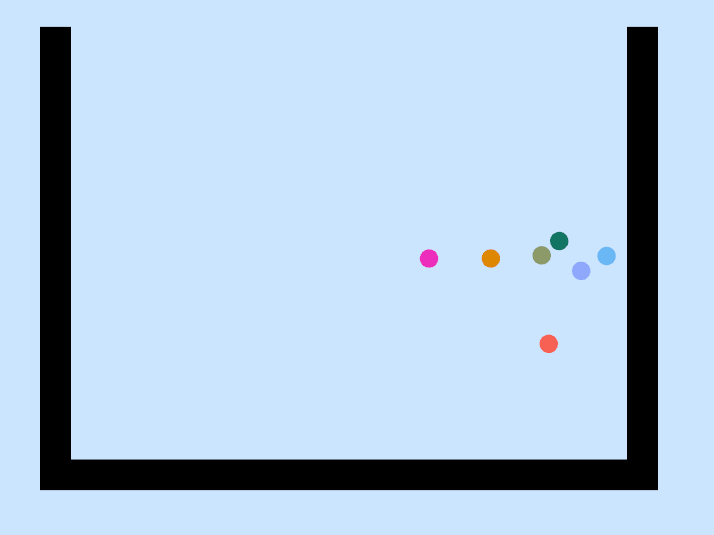
\includegraphics[width=\linewidth, width=60mm]{bilder/OpenGL_bounce1.png}
      \centering
      \captionof{figure}{Seven bouncing weights in a room}
    \end{minipage} 
  \end{tabular}
\end{table}

In the first part, the pendulums were affected by air resistance. In this scene the balls have the properties of lead and the air resistance coefficient was calculated from the circular shape. 


\section{Discussion}
The implementation of the physics into code started as soon as the idea was found which made this project robust and stable from the beginning.
The work was most of the time divided into groups of two and these pairs implemented and discussed code together which made the work hours efficient.

During the conversion to C++, a couple of obstacles in terms of different operative systems and the different versions of OpenGL caused troubles. This took much time and focus from the project itself. OpenGL 3.3 has some new implementations when drawing objects, different from what we have used before.

The Euler explicit method was first used as the numerical integration method. However, Euler gives a larger numerical error which grows for each iteration. This is noticeable when using a larger step size since the simulation gets unstable. To minimize this problem the Runge-Kutta 4 method was implemented, which represent a more accurate model. This method considers four following steps, each dependent on the previous one, from which a weighted average representing the next step of the slope could be calculated. 

Another difficulty with the simulation was to handle time as a parameter. In this project the simulation was performed as fast as the current computer could compute the code, which brought troubles with different computers. Some computers calculated the code too fast and in that case the simulation could look unrealistic.

One idea was to implement a simple model so that the balls could roll off each other to avoid the scenario that weights gets stuck on top of each other at low velocities. However, this was not implemented due to lack of time. 

\newpage
\bibliography{angrybib}
\bibliographystyle{plain}

\newpage
\pagenumbering{gobble}
\section*{Appendix 1}


\begin{center}
\begin{table}[!ht]
\captionsetup{justification=raggedright, singlelinecheck=false}
\caption{Constants for the weights}
	\begin{tabular}{| l | l  c |}
		\hline
		\multicolumn{3}{| c |}{CONSTANTS} \\ \hline
		Radius & $0.02$ &$(m)$ \\ \hline
		Volume & $1.68*10^{-5}$ & $(m^{3})$ \\ \hline
		Density & $11340$ & $(kg/m^{3})$ \\ \hline
		Mass & $0.19$ & $(kg)$ \\ \hline
		Air Coefficient & $0.47$ & \\ \hline
	\end{tabular}
\end{table}
\end{center}

\end{document}

